\documentclass[12pt,letterpaper]{article}
\usepackage{graphicx,textcomp}
\usepackage{natbib}
\usepackage{setspace}
\usepackage{fullpage}
\usepackage{color}
\usepackage[reqno]{amsmath}
\usepackage{amsthm}
\usepackage{fancyvrb}
\usepackage{amssymb,enumerate}
\usepackage[all]{xy}
\usepackage{endnotes}
\usepackage{lscape}
\newtheorem{com}{Comment}
\usepackage{float}
\usepackage{hyperref}
\newtheorem{lem} {Lemma}
\newtheorem{prop}{Proposition}
\newtheorem{thm}{Theorem}
\newtheorem{defn}{Definition}
\newtheorem{cor}{Corollary}
\newtheorem{obs}{Observation}
\usepackage[compact]{titlesec}
\usepackage{dcolumn}
\usepackage{tikz}
\usetikzlibrary{arrows}
\usepackage{multirow}
\usepackage{xcolor}
\newcolumntype{.}{D{.}{.}{-1}}
\newcolumntype{d}[1]{D{.}{.}{#1}}
\definecolor{light-gray}{gray}{0.65}
\usepackage{url}
\usepackage{listings}
\usepackage{color}

\definecolor{codegreen}{rgb}{0,0.6,0}
\definecolor{codegray}{rgb}{0.5,0.5,0.5}
\definecolor{codepurple}{rgb}{0.58,0,0.82}
\definecolor{backcolour}{rgb}{0.95,0.95,0.92}

\lstdefinestyle{mystyle}{
	backgroundcolor=\color{backcolour},   
	commentstyle=\color{codegreen},
	keywordstyle=\color{magenta},
	numberstyle=\tiny\color{codegray},
	stringstyle=\color{codepurple},
	basicstyle=\footnotesize,
	breakatwhitespace=false,         
	breaklines=true,                 
	captionpos=b,                    
	keepspaces=true,                 
	numbers=left,                    
	numbersep=5pt,                  
	showspaces=false,                
	showstringspaces=false,
	showtabs=false,                  
	tabsize=2
}
\lstset{style=mystyle}
\newcommand{\Sref}[1]{Section~\ref{#1}}
\newtheorem{hyp}{Hypothesis}

\title{Problem Set 1}
\date{Due: October 1, 2023}
\author{Applied Stats/Quant Methods 1}

\begin{document}
	\maketitle
	
	\section*{Instructions}
	\begin{itemize}
	\item Please show your work! You may lose points by simply writing in the answer. If the problem requires you to execute commands in \texttt{R}, please include the code you used to get your answers. Please also include the \texttt{.R} file that contains your code. If you are not sure if work needs to be shown for a particular problem, please ask.
\item Your homework should be submitted electronically on GitHub.
\item This problem set is due before 23:59 on Sunday October 1, 2023. No late assignments will be accepted.
\item Total available points for this homework is 80.
	\end{itemize}
	
	\vspace{1cm}
	\section*{Question 1 (40 points): Education}

A school counselor was curious about the average of IQ of the students in her school and took a random sample of 25 students' IQ scores. The following is the data set:\\
\vspace{.5cm}

\lstinputlisting[language=R, firstline=36, lastline=36]{PS01.R}  

\vspace{1cm}

\begin{enumerate}
	\item Find a 90\% confidence interval for the average student IQ in the school.\\
	
	\item Next, the school counselor was curious  whether  the average student IQ in her school is higher than the average IQ score (100) among all the schools in the country.\\ 
	
	\noindent Using the same sample, conduct the appropriate hypothesis test with $\alpha=0.05$.
\end{enumerate}

\newpage

	\vspace{1cm}
\section*{Answers Q1 (part 1)}


\noindent To find the 90 per cent Confidence Interval, we look for the Point estimate +/- Margin of error, where margin of error is a multiple of the standard error.\\

\noindent What do we need? \\

1. Central tendency, mean - a point estimate: mean(y)  \\ 

2. Variability, the standard error:  sd(y) / sqrt(length(y)) \\

\noindent Looking at the normal distribution, we see that 90 per cent of observations lie within +/-1.64 standard errors of the point estimate \\

\begin{verbatim}
qnorm(0.05) # value for first 5% 
qnorm(0.95) # value last 5% 
\end{verbatim}

\noindent Solution method 1: The **approximate** solution for 90 per cent confidence level \\

\begin{verbatim}
upper_90 = mean(y)+(1.64*sd(y) / sqrt(length(y)))
lower_90 = mean(y)-(1.64*sd(y) / sqrt(length(y)))
\end{verbatim}

\noindent 90 per cent confidence level calculated as 94.14554 to 102.7345 \\

\noindent Solution method 2: The **precise** solution for 90 per cent confidence level \\

\begin{verbatim}
lower_90_n <- qnorm(0.05, 
mean = mean(y), 
sd = (sd(y) / sqrt(length(y))))

upper_90_n <- qnorm(0.95,
mean = mean(y),
sd = (sd(y) / sqrt(length(y))))
\end{verbatim}

\noindent  \textbf {On this basis, we can confirm that the confidence interval lies between 94.13283 and 102.7472}
 
\newpage

\section*{Answers Q1 (part 2)}

\noindent  As the sample size is less than 30 we conduct a T-test. It will be a one-sided test as we are looking to see if the student IQ in the school is higher than the population average. \\

The NULL Hypothesis is that there is no difference. \\

The Alternative Hypothesis is that the IQ is higher in the school \\

The significance level is set at 0.05 \\

First step: calculate the standard error, T-statistic, and probability score: 

\begin{verbatim}
standard_error <-  sd(y) / sqrt(length(y))
t_statistic <- abs((mean(y) - 100) / standard_error)
prob <- pt(t_statistic, (length(y)-1))
\end{verbatim}

P VALUE = 0.7215383 \\

\noindent \textbf {Therefore we have evidence to accept the null hypothesis, as the p value is greater than 0.05.} \\

\\

\noindent Alternatively, we can find the same result using the below method: 

\begin{verbatim}
t.test(y, mu = 100, conf.level = 0.05, alternative = "greater")
\end{verbatim}

This gives the same P VALUE

\newpage

	\section*{Question 2 (40 points): Political Economy}
	




\noindent Researchers are curious about what affects the amount of money communities spend on addressing homelessness. The following variables constitute our data set about social welfare expenditures in the USA. \\
\vspace{.5cm}


\begin{tabular}{r|l}
	\texttt{State} &\emph{50 states in US} \\
	\texttt{Y} & \emph{per capita expenditure on shelters/housing assistance in state}\\
	\texttt{X1} &\emph{per capita personal income in state} \\
	\texttt{X2} &  \emph{Number of residents per 100,000 that are "financially insecure" in state}\\
	\texttt{X3} &  \emph{Number of people per thousand residing in urban areas in state} \\
	\texttt{Region} &  \emph{1=Northeast, 2= North Central, 3= South, 4=West} \\
\end{tabular}

\vspace{.5cm}
\noindent Explore the \texttt{expenditure} data set and import data into \texttt{R}.
\vspace{.5cm}
\lstinputlisting[language=R, firstline=54, lastline=54]{PS01.R}  
\vspace{.5cm}
\begin{itemize}

\item
Please plot the relationships among \emph{Y}, \emph{X1}, \emph{X2}, and \emph{X3}? What are the correlations among them (you just need to describe the graph and the relationships among them)?
\vspace{.5cm}
\item
Please plot the relationship between \emph{Y} and \emph{Region}? On average, which region has the highest per capita expenditure on housing assistance?
\vspace{.5cm}
\item
Please plot the relationship between \emph{Y} and \emph{X1}? Describe this graph and the relationship. Reproduce the above graph including one more variable \emph{Region} and display different regions with different types of symbols and colors.
\end{itemize}

\newpage

	\section*{Answers Q2 (part 1)}
	
	

\noindent 


\begin{figure}[H] % Place figure here
	
	\centering
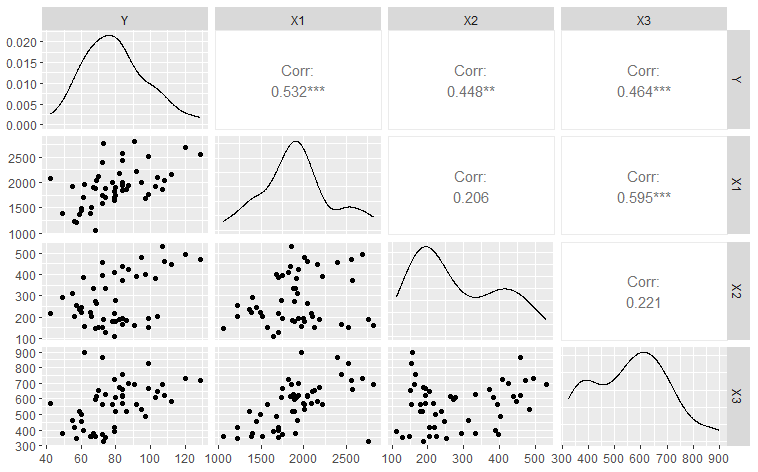
\includegraphics[scale=0.75]{Rplot06_GG.png}
\caption{Scatter Plots with Correlation}
\label{fig:scatterplot}
\newpage
\end{figure} 
	
\begin{tabular}{r|l}
	\texttt{Y} & \emph{per capita expenditure on shelters/housing assistance in state}\\
	\texttt{X1} &\emph{per capita personal income in state} \\
	\texttt{X2} &  \emph{Number of residents per 100,000 that are "financially insecure" in state}\\
	\texttt{X3} &  \emph{Number of people per thousand residing in urban areas in state} \\
\end{tabular} \\

\
\

\noindent The strongest associations observed are between per capital expenditure on shelters/housing assistance in the state (Y) and per capita personal income in state (X1) and also between Y and the number of people living in urban areas in the state (X3). \\

\noindent The weakest associations are between the per capital personal income in state (X1) and number of residents per 100,00 that are "financially secure" in state (X2), as well as between number of residents that are financially secure (X2) and the number of people residing in urban areas of the state (X3).\\

\newpage

\section*{Answers Q2 (part 2)}

\begin{figure}[H] % Place figure here
	
	\centering
	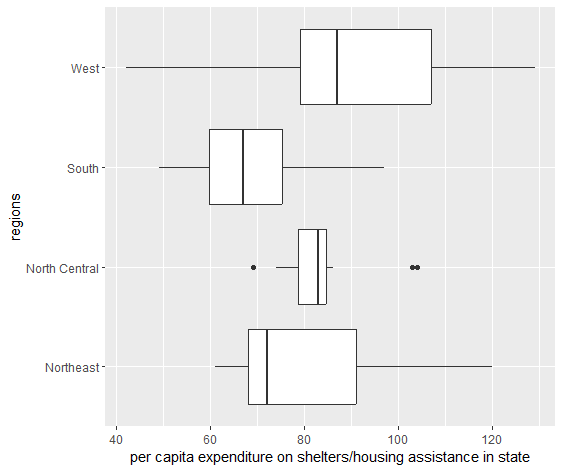
\includegraphics[scale=1.0]{Rplot_box_2.png}
	\caption{Comparison of State Expenditure on shelters by regions}
	\label{fig: boxplot}
	\newpage
\end{figure} 


\noindent  \textbf {Comment: the West region appears to have the highest expenditure on shelters / housing assistance.}


\newpage

\section*{Answers Q2 (part 3)}


\begin{figure}[H] % Place figure here
	
	\centering
	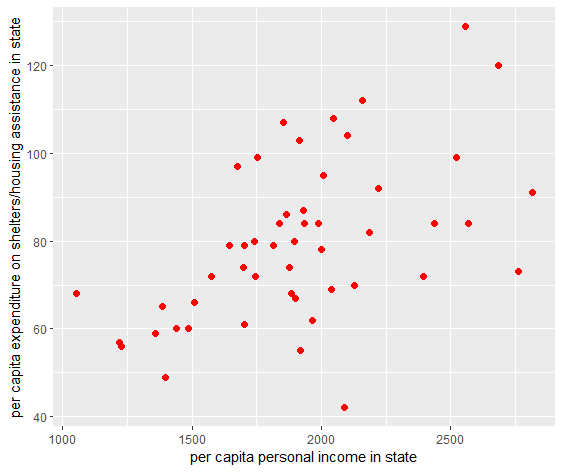
\includegraphics[scale=0.5]{Rplot07_red.png}
	\caption{Comparison of State Expenditure with Personal Income}
	\label{fig:scatterplot}
	\newpage
\end{figure} 


\begin{figure}[H] % Place figure here
	
	\centering
	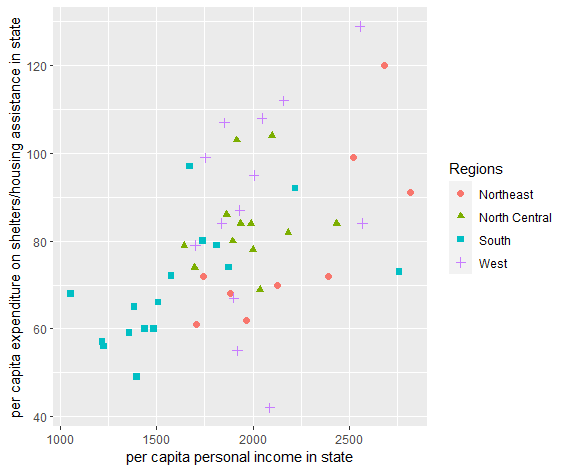
\includegraphics[scale=0.5]{Rplot_with_regions.png}
	\caption{Association across Regions}
	\label{fig:scatterplot}
	\newpage
\end{figure} 

\noindent  \textbf {There is a strong correlation in Figure 3 (calculated to be 0.532). In Figure 4, you can see a strong correlation in particular across the Southern region and the North Central region. The Northeast and Western regions appear to have a less strong correlation.}

\end{document}


